%!TEX TS-program = xelatex
%!TEX encoding = UTF-8 Unicode

%%%%%%%%%%%% 选择学位类型：博士、学硕%%%%%%%%%%%
\documentclass[Bachelor]{DLUT-thesis}  %%学硕
\usepackage[T1]{fontenc}  %设置英文字体为times new roman
\usepackage{mathptmx}
\usepackage{caption}
\usepackage{tikz}
\usetikzlibrary{arrows.meta}


%%%%%%%%%%%%%%%%填写封面信息%%%%%%%%%%%%%%%%%%%%%%%%

%论文题目
\title{大连理工大学本科毕业论文（设计）}
%论文题目中文
\chinesetitle{基于强化学习的特种机器人环境自适应变体控制}
%论文题目英文
\englishtitle{Environment-Adaptive Morphological Control for Specialized Robots Based on Reinforcement Learning}  
%论文题目日文
% \japanesetitle{大連理工大学卒業論文タイトル}  

\institute{机械工程学院~~~~~~~~~~~~~~~~~~~~~~~~~~~~~~~~~~~~~~~~~~~~~~~}                %学院
\dutmajor{机械设计制造及其自动化（日语强化）~~~~~~~~~~~~~~~~~~~~~~~~~~~}                 %专业
\author{刘倍佐~~~~~~~~~~~~~~~~~~~~~~~~~~~~~~~~~~~~~~~~~~~~~~~~~~~~~~~~~~~~~~~~}       %作者姓名
\studentNumber{20221043011~~~~~~~~~~~~~~~~~~~~~~~~~~~~~~~~~~~~~~~~~~~~~~~~~~~~~~~~~}  %作者学号
\advisor{李海洋~~~~~~~~~~~~~~~~~~~~~~~~~~~~~~~~~~~~~~~~~~~~~~~~~~~~~~~~~~~~~}         %导师姓名
\reviewer{Prof. XXX~~~~~~~~~~~~~~~~~~~~~~~~~~~~~~~~~~~~~~~~~~~~~~~~~~~~~~~~~~}		  %评阅教师姓名
\datetime{~~~~~~~~~~~~~~~~~~~~~~~~~~~~~~~~~~~~~~~~~~~~~~~~~~~~~~~~~}        %编辑日期

%%%%%%%%%%%%%%%%%%%%%%%%%%%%%%%%%%%%%%%%%%%%%%
%\setmainfont{Times New Roman}

\begin{document}

% \captionsetup[figure]{labelformat={default}, labelsep=space, name={Figure}}
% \captionsetup[table]{labelformat={default}, labelsep=space, name={Table}}
\captionsetup[figure]{labelformat=simple, labelsep=space, name={Figure}}
\captionsetup[table]{labelformat=simple, labelsep=space, name={Table}}

	\makeDUTCover
	\makeAuthorization

	
	\include{chapters/abstract}   								 %中文摘要
	 \setlength{\baselineskip}{20pt}
\begin{englishabstract}

	\centerline{\zihao{-3}{Abstract}}\par
	~\par
	\zihao{-4}

	外文摘要要求用英文书写，内容应与“中文摘要”对应。使用第三人称，最好采用现在时态编写。\par
	“Abstract”不可省略。标题“Abstract”选用模板中的样式所定义的“标题1”，再居中；或者手动设置成字体：Times New Roman，居中，字号：小三，多倍行距1.5倍行距，段后11磅，段前为0行。\par
	标题“Abstract”上方是论文的英文题目，字体：Times New Roman，居中，字号：小三，行距：多倍行距 1.25，间距：段前、段后均为0行，取消网格对齐选项。\par
	Abstract正文选用设置成每段落首行缩进2字，字体：Times New Roman，字号：小四，行距：多倍行距 1.25，间距：段前、段后均为0行，取消网格对齐选项。\par
	Key words与摘要正文之间空一行。Key words与中文“关键词”一致。词间用分号间隔，末尾不加标点，3-5个；Times New Roman，小四，加粗。\par
	
	~\par
	\noindent\englishkeywords{\bfseries Write Criterion; Typeset Format; Graduation Project (Thesis)}

\end{englishabstract}  						 %英文摘要
	% \include{chapters/japaneseabstract}  						 %日文摘要


	\tableofcontents
    % 手动设置第二页的页面样式为 DLUT@heading
    \thispagestyle{DLUT@heading}
    \newpage\pagenumbering{arabic}

	\pagestyle{DLUT@heading}
    %正文部分
 	%\include{chapters/preface} 									%引言 
    \setlength{\baselineskip}{20pt}
\chapter{Introduction}
\label{cha:conintro}
\zihao{-4}

The superhydrophobic surface is defined as the surface with the contact angle between water more than 150. It has essential application in self-cleaning, drag reduction, corrosion resistance, etc \cite{fang2015survey}\cite{MATSUMURA2017566}. 

This chapter will introduce the research background of superhydrophobic surfaces on metal substrates and its significance, analyze the existed preparation method of superhydrophobic surfaces and their problems, and finally briefly expound the research target and the main contents of this thesis.

说明：

(1)	标题字号及行距按照模板。

(2)	正文采用1.25倍行距，段前段后均为0，取消网格对齐选项。小四字号，Times New Roman。

(3)	图、表、公式参照模板格式。

(4)	论文类10000-12500单词（正文45-60页），公式、图标不计入单词数。

\section{Research background and significance}

\begin{figure}[!htb] % use float package if you want it here
    %\setlength{\abovecaptionskip}{-0.2cm} %调整图片caption与正文之间的间距，table同理。可自己调整。
    \setlength{\belowcaptionskip}{-0.2cm} 
      \centering
      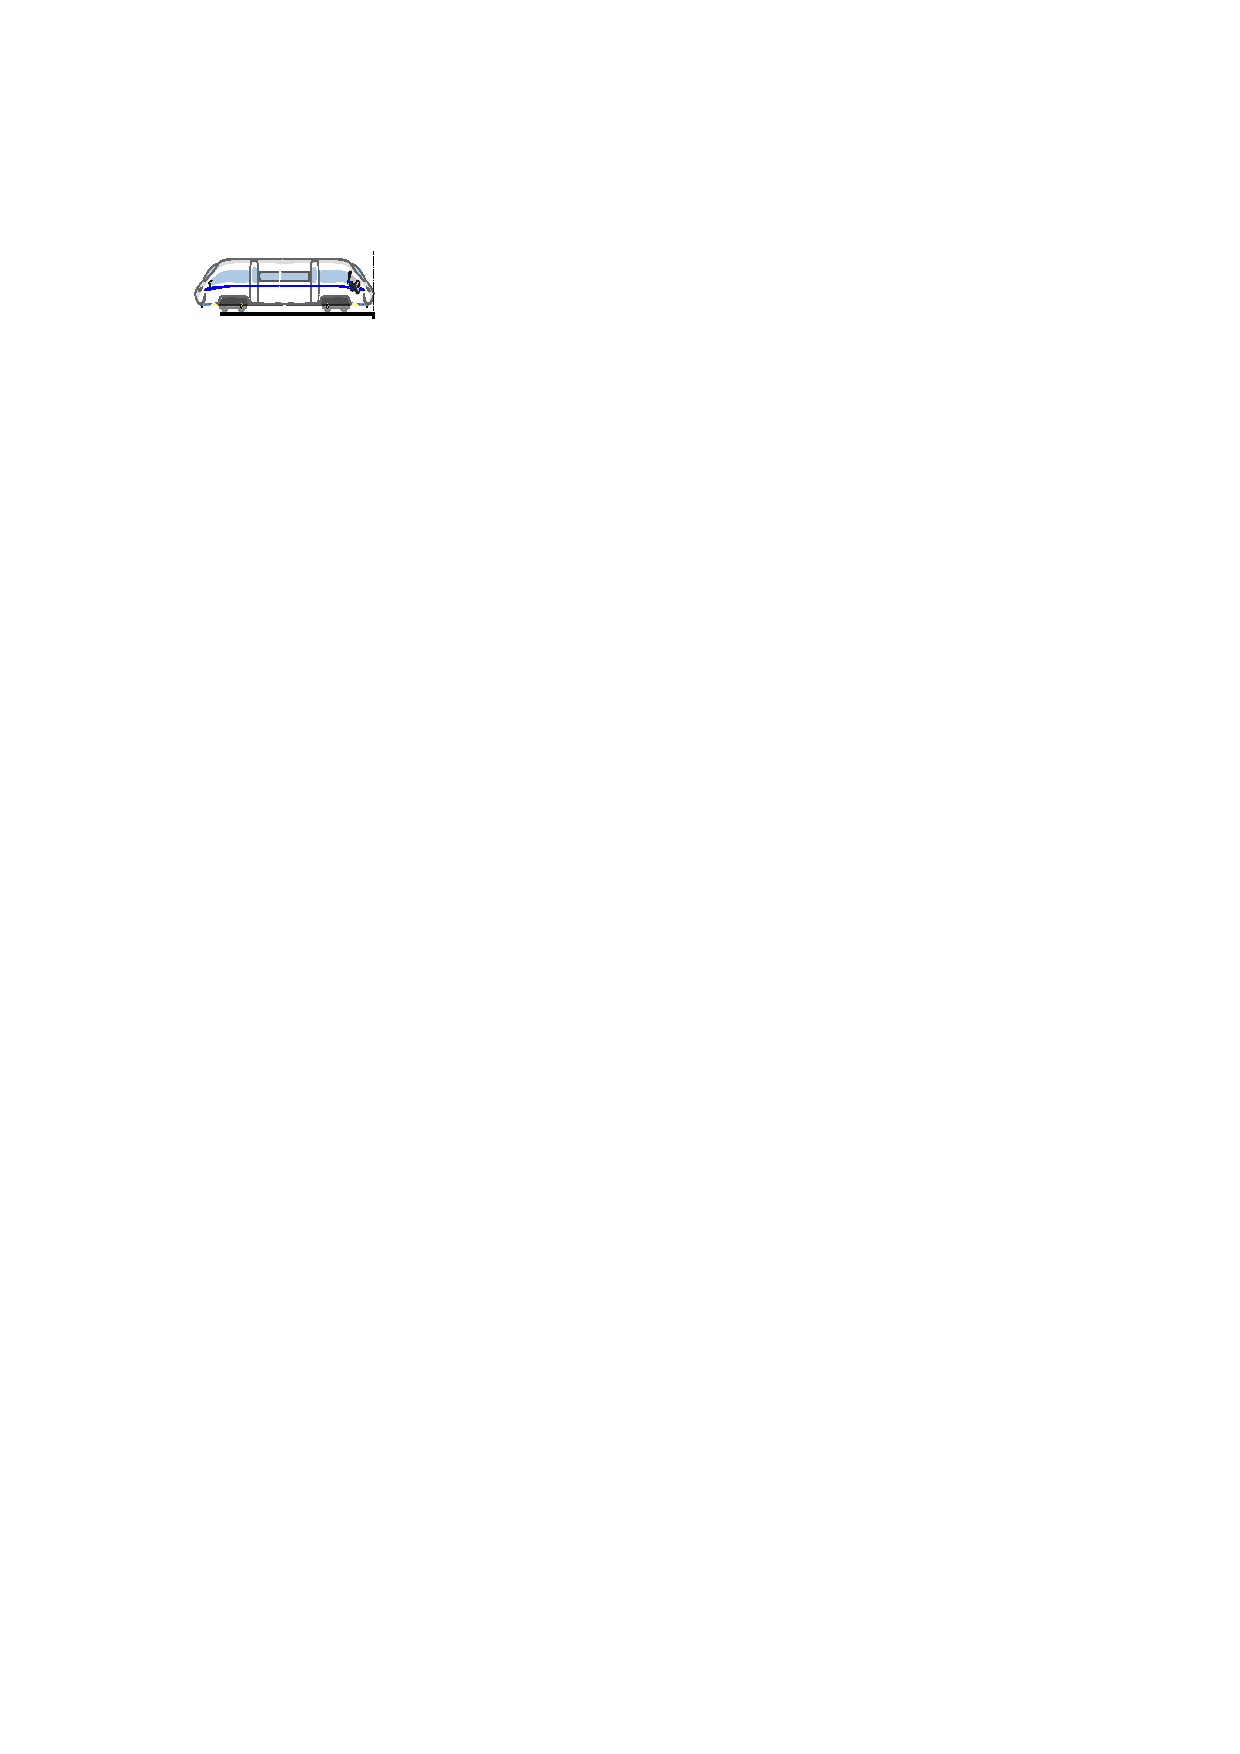
\includegraphics[scale=1]{figures/figure1.pdf}
      \caption{Figure title}
      \label{fig:01:01}
\end{figure}

\section{The research status of superhydrophobic surfaces}

\subsection{International status for theoretical research}

\subsection{Domestic status for theoretical research}

\subsection{Existed method of fabrication of superhydrophobic surface}

\section{The problems of existed methods of superhydrophobic surface}

\section{Research target and main content}

\section{Summary}



 								%第一章
    \setlength{\baselineskip}{20pt}
\chapter{Relevant Theories on Metal Superhydrophobic Surface}
\label{cha:chap2}

\section{Classical theoretical model of wettability}

\subsection{Young model}


\begin{figure}[!htb] % use float package if you want it here
%\setlength{\abovecaptionskip}{-0.2cm} %调整图片caption与正文之间的间距，table同理。可自己调整。
\setlength{\belowcaptionskip}{-0.2cm} 
  \centering
  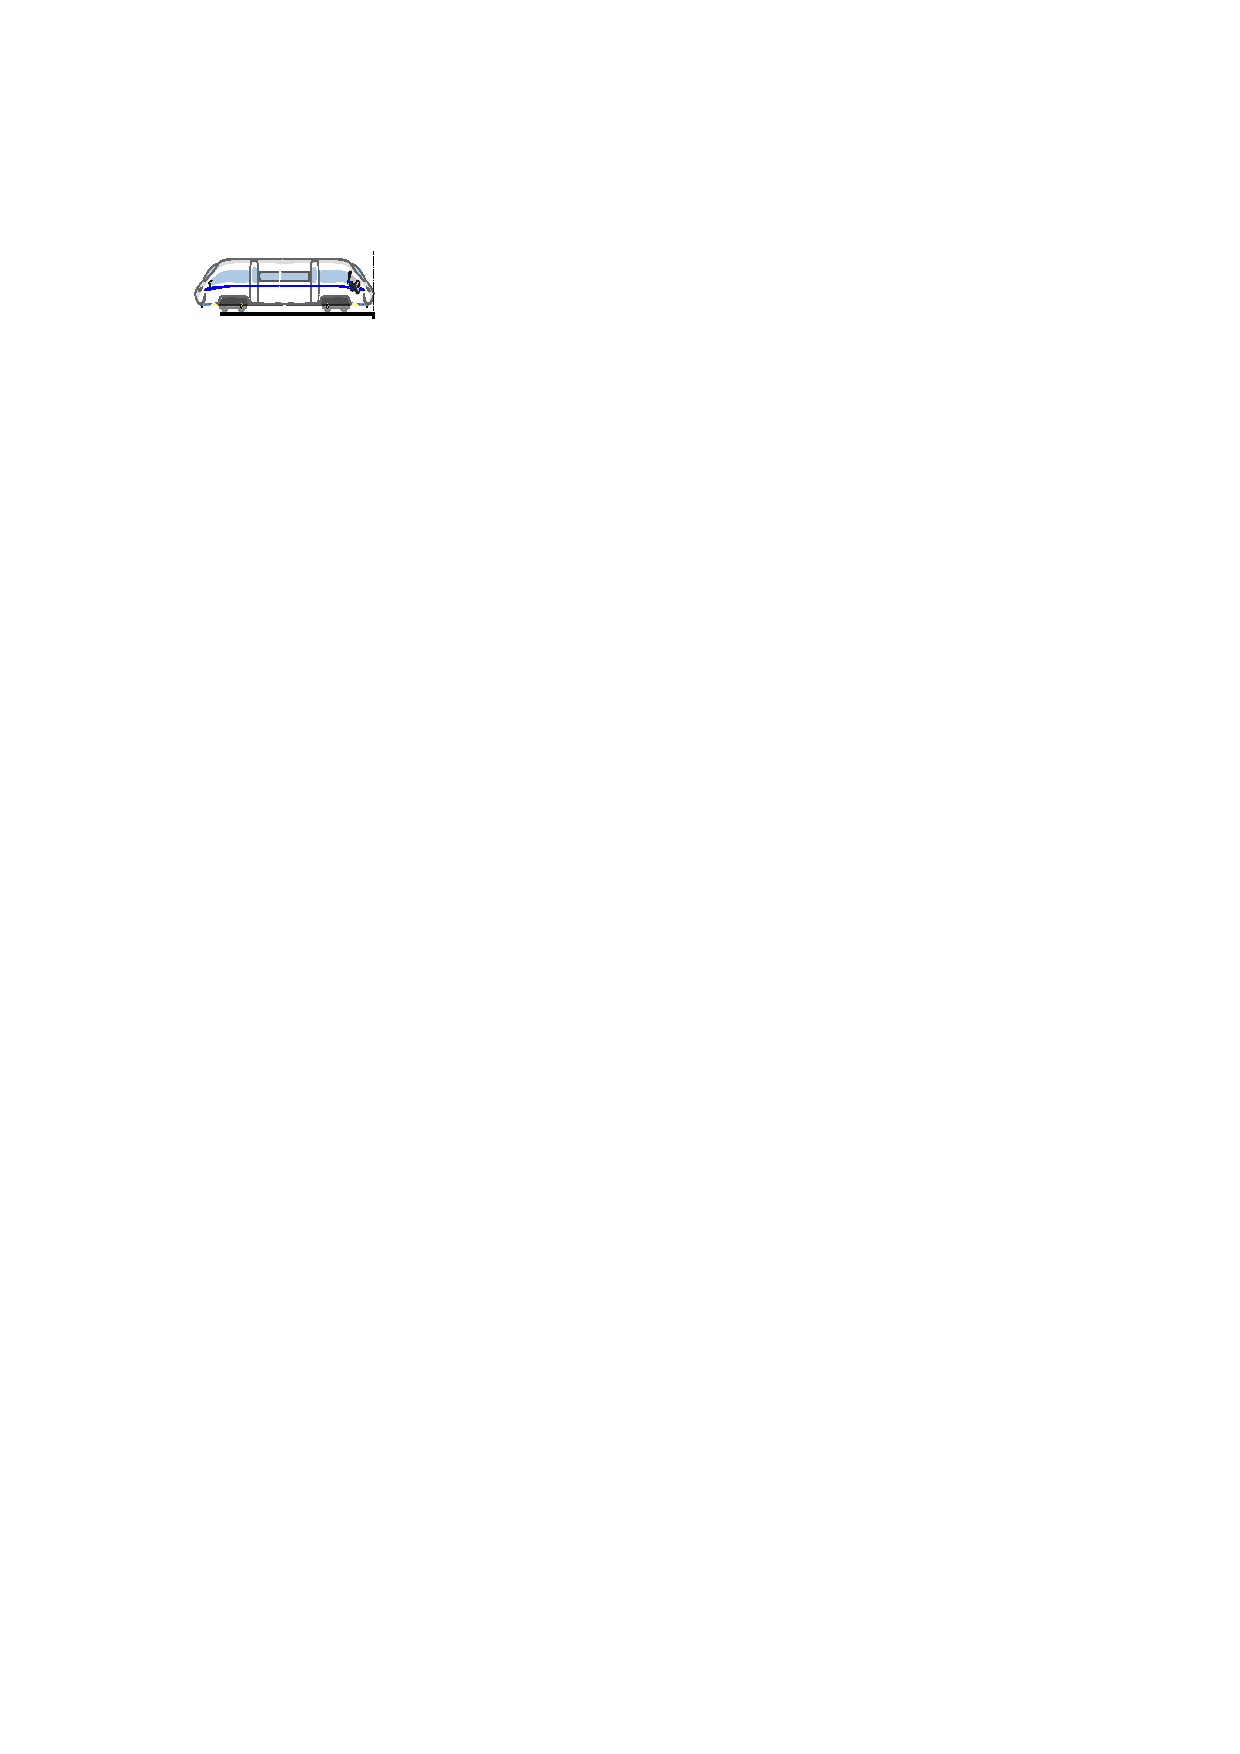
\includegraphics[scale=1]{figures/figure1.pdf}
  \caption{示例图片。}
  \label{fig:02:01}
\end{figure}


例如：如表格\ref{table:02:01}所示

\begin{table}[!htb]\small   %%\small是为了设置表格中的字体比正文小
\setlength{\abovecaptionskip}{-0.05cm} %调整图片caption与正文之间的间距，table同理。可自己调整。
\setlength{\belowcaptionskip}{-0.2cm} 
  \centering
  \renewcommand\arraystretch{1}
  \caption{示例表格。}

 \begin{tabular}{p{1cm} p{1cm}<{\centering} p{1cm}<{\centering} p{1cm}<{\centering} p{1cm}<{\centering} p{1cm}<{\centering}  }
  \hline
  AA &
  BB &
  CC &
  DD &
  EE &
  FF
  \\
  \hline
    AA   &  1.1   & 1.1 & 1.1 & 1.1&  1.1    \\
    BB   &  1.1   & 1.1 & 1.1 & 1.1&  1.1    \\
    CC   &  1.1   & 1.1 & 1.1 & 1.1&  1.1   \\
  \hline
  \end{tabular}
  \label{table:02:01}
\end{table}


单独为行公式示例：如公式\ref{eq:02:01}，公式\ref{eq:02:02a}所示。

\begin{equation}\label{eq:02:01}
\left\{
\begin{split}
\frac{\texttt{d}p(t)}{\texttt{d}t}&=v(t)\\
\frac{\texttt{d}v(t)}{\texttt{d}t}&=u(t)-a(t)-b(t)v(t)-c(t)v^2(t)-f_2^*(\cdot)
\end{split}
\right.
\end{equation}


\begin{subequations}\label{eq:02:02}
  \begin{align}
  \dot{\hat{A}}^\dag&=\lambda_1\left(\tanh(k_3e_v)e_v-\sigma_1\hat{A}^\dag\right)\label{eq:02:02a}\\
  \dot{\hat{b}}^\dag&=\lambda_2\left(|v||e_v|-\sigma_2\hat{b}^\dag\right)\label{eq:02:02b}\\
  \dot{\hat{c}}^\dag&=\lambda_3\left(v^2|e_v|-\sigma_3\hat{c}^\dag\right)\label{eq:02:02c}
  \end{align}
  \end{subequations}

嵌入在文本中的公式例子：$a + b = c$。

\subsection{Wenzel model}

\subsection{Cassie-Baxter model}

\section{Summary}




%\bibliography{reference/ref.bib}


 								%第二章
	\setlength{\baselineskip}{20pt}
\chapter{球铰等效机构逆运动学建模}
\label{cha:chap3}

\section{逆运动学推导基础}

\subsection{三维旋转矩阵}

本文研究对象可抽象为以公共球心 $O$ 为旋转中心的球面机构，因此其位姿变化本质上是刚体绕固定点的三维转动。为避免符号混淆，动平台姿态采用滚转角 $\phi$、俯仰角 $\vartheta$ 和偏航角 $\psi$ 表示，主动关节输入角采用 $\theta_i$ 表示，其中 $i=1,2,3$。在右手坐标系和列向量表示下，绕 $x$、$y$、$z$ 轴的基本旋转矩阵分别为
\begin{equation}
R_x(\phi)=
\begin{bmatrix}
1 & 0 & 0 \\
0 & \cos\phi & -\sin\phi \\
0 & \sin\phi & \cos\phi
\end{bmatrix}
\label{eq:03:rx}
\end{equation}

\begin{equation}
R_y(\vartheta)=
\begin{bmatrix}
\cos\vartheta & 0 & \sin\vartheta \\
0 & 1 & 0 \\
-\sin\vartheta & 0 & \cos\vartheta
\end{bmatrix}
\label{eq:03:ry}
\end{equation}

\begin{equation}
R_z(\psi)=
\begin{bmatrix}
\cos\psi & -\sin\psi & 0 \\
\sin\psi & \cos\psi & 0 \\
0 & 0 & 1
\end{bmatrix}
\label{eq:03:rz}
\end{equation}

若向量 $a$ 在坐标系 $\{B\}$ 中的表示为 $a^B$，则其在坐标系 $\{A\}$ 中的表示满足
\begin{equation}
a^A = R_A^B a^B
\label{eq:03:vector_transform}
\end{equation}
因此，逆运动学推导的核心就是建立各局部坐标系到基坐标系的旋转映射关系，并从旋转后的方向向量中提取主动关节角。

\subsection{齐次变换矩阵}

一般刚体位姿既包含方向也包含位置，统一表达方式为齐次变换矩阵
\begin{equation}
T_A^B=
\begin{bmatrix}
R_A^B & p_A^B \\
0\ 0\ 0 & 1
\end{bmatrix}
\label{eq:03:htm_general}
\end{equation}
式中，$R_A^B$ 表示坐标系 $\{B\}$ 相对 $\{A\}$ 的姿态，$p_A^B$ 表示坐标系 $\{B\}$ 原点在 $\{A\}$ 中的位置。

对于 3-RRR 球面并联机构，所有转轴均交于公共点 $O$，动平台仅发生绕该点的转动而不存在平移自由度，因此可将式 \eqref{eq:03:htm_general} 简化为
\begin{equation}
T_A^B=
\begin{bmatrix}
R_A^B & 0 \\
0\ 0\ 0 & 1
\end{bmatrix}
\label{eq:03:htm_spherical}
\end{equation}
这意味着本文的逆运动学问题可以完全转化为姿态矩阵与方向余弦向量之间的关系求解，而不必额外处理末端位置变量。

\subsection{球面机构的方向向量约束}

3-RRR 球面并联机构的每条支链均由主动转轴、近端转轴和远端转轴组成。设三类转轴在基坐标系中的单位方向向量分别为 $u_i$、$w_i$ 和 $v_i$，则由球面机构的几何约束可知，$w_i$ 与 $v_i$ 的夹角恒为结构常数 $\alpha_2$，因此满足
\begin{equation}
w_i^{\mathrm{T}} v_i = \cos\alpha_2,\quad i=1,2,3
\label{eq:03:dot_constraint}
\end{equation}
式 \eqref{eq:03:dot_constraint} 是后续逆运动学闭式求解的出发点。只要将 $w_i$ 和 $v_i$ 分别表示为主动关节角与末端姿态角的函数，就可以把机构几何约束转写为关于 $\theta_i$ 的代数方程。

\section{3-RRR 球面并联机构逆运动学推导}

参考文献 \cite{sadeqi2017} 给出了 3-RRR 球面并联机构的经典逆运动学求解框架。结合本文球铰等效机构的坐标定义以及符号化校核结果，现将与后续仿真模型一致的推导过程整理如下。

\subsection{机构参数与主动关节轴向量}

设 $\eta_i$ 表示第 $i$ 条支链在基坐标系 $x$-$y$ 平面内的方位角，$\gamma$ 表示主动转轴与全局 $z$ 轴之间的夹角，$\alpha_1$ 表示主动转轴与近端转轴之间的夹角，$\beta$ 表示机构处于零位时远端转轴相对全局 $z$ 轴的夹角。记
\begin{equation}
e_x=
\begin{bmatrix}
1 \\ 0 \\ 0
\end{bmatrix}
\label{eq:03:ex}
\end{equation}
则第 $i$ 条支链主动关节轴对应的姿态变换可写为
\begin{equation}
R_{01}^{(i)} = R_z\left(\eta_i + \frac{\pi}{2}\right) R_y\left(\frac{\pi}{2} - \gamma\right)
\label{eq:03:r01}
\end{equation}
主动关节轴方向向量即为该矩阵的第一列
\begin{equation}
u_i = R_{01}^{(i)} e_x =
\begin{bmatrix}
-\sin\eta_i \sin\gamma \\
\cos\eta_i \sin\gamma \\
-\cos\gamma
\end{bmatrix}
\label{eq:03:ui}
\end{equation}

\subsection{近端转轴方向向量}

在第 $i$ 条支链中，近端转轴方向向量 $w_i$ 由两步旋转得到。第一步绕局部 $x$ 轴转动主动关节角 $\theta_i$；第二步绕更新后的局部 $z$ 轴转动结构角 $\alpha_1$。因此局部旋转矩阵为
\begin{equation}
R_{\mathrm{loc}}^{(i)} = R_x(\theta_i) R_z(\alpha_1)
\label{eq:03:rloc}
\end{equation}
将其映射到基坐标系可得
\begin{equation}
R_w^{(i)} = R_{01}^{(i)} R_{\mathrm{loc}}^{(i)}
\label{eq:03:rw}
\end{equation}
于是，近端转轴方向向量写为
\begin{equation}
w_i = R_w^{(i)} e_x
\label{eq:03:wi_def}
\end{equation}
展开后得到
\begin{equation}
w_i =
\begin{bmatrix}
-\cos\eta_i \sin\alpha_1 \cos\theta_i - \cos\alpha_1 \sin\eta_i \sin\gamma - \cos\gamma \sin\alpha_1 \sin\eta_i \sin\theta_i \\
\cos\alpha_1 \cos\eta_i \sin\gamma - \sin\alpha_1 \cos\theta_i \sin\eta_i + \cos\eta_i \cos\gamma \sin\alpha_1 \sin\theta_i \\
\sin\alpha_1 \sin\gamma \sin\theta_i - \cos\alpha_1 \cos\gamma
\end{bmatrix}
\label{eq:03:wi}
\end{equation}

\subsection{动平台远端转轴方向向量}

为了建立末端姿态与远端转轴方向之间的关系，先定义机构零位下第 $i$ 条支链远端转轴的参考姿态矩阵。按照本文坐标约定，其表达式取为
\begin{equation}
R_{03}^{(i)} = R_z\left(\eta_i + \frac{5\pi}{6}\right) R_y\left(\beta - \frac{\pi}{2}\right)
\label{eq:03:r03}
\end{equation}

动平台相对基坐标系的姿态采用固定轴 ZYX 旋转序列表示，即
\begin{equation}
R_{rpy} = R_z(\psi) R_y(\vartheta) R_x(\phi)
\label{eq:03:rrpy}
\end{equation}
于是，末端姿态作用后的远端转轴方向向量为
\begin{equation}
v_i = R_{rpy} R_{03}^{(i)} e_x =
\begin{bmatrix}
v_{ix} \\
v_{iy} \\
v_{iz}
\end{bmatrix}
\label{eq:03:vi}
\end{equation}
式中，$v_{ix}$、$v_{iy}$ 和 $v_{iz}$ 是 $\phi$、$\vartheta$、$\psi$、$\beta$ 与 $\eta_i$ 的函数。由于其完整展开式较长，后续推导保留分量形式，以便直接整理出关于 $\theta_i$ 的闭式方程。

\subsection{约束方程整理与闭式求解}

将式 \eqref{eq:03:wi} 和式 \eqref{eq:03:vi} 代入几何约束式 \eqref{eq:03:dot_constraint}，可以得到关于主动关节角 $\theta_i$ 的三角方程
\begin{equation}
a_i \sin\theta_i + b_i \cos\theta_i + d_i = 0
\label{eq:03:trig_constraint}
\end{equation}
其中
\begin{equation}
a_i = \sin\alpha_1 \left( v_{iz}\sin\gamma + v_{iy}\cos\eta_i\cos\gamma - v_{ix}\cos\gamma\sin\eta_i \right)
\label{eq:03:a}
\end{equation}

\begin{equation}
b_i = -\sin\alpha_1 \left( v_{ix}\cos\eta_i + v_{iy}\sin\eta_i \right)
\label{eq:03:b}
\end{equation}

\begin{equation}
d_i = v_{iy}\cos\alpha_1\cos\eta_i\sin\gamma - v_{iz}\cos\alpha_1\cos\gamma - \cos\alpha_2 - v_{ix}\cos\alpha_1\sin\eta_i\sin\gamma
\label{eq:03:d}
\end{equation}

为将式 \eqref{eq:03:trig_constraint} 化为代数方程，令
\begin{equation}
t_i = \tan\frac{\theta_i}{2}
\label{eq:03:half_angle}
\end{equation}
则有
\begin{equation}
\sin\theta_i = \frac{2t_i}{1+t_i^2}, \qquad
\cos\theta_i = \frac{1-t_i^2}{1+t_i^2}
\label{eq:03:half_angle_expand}
\end{equation}
代入并整理后，可得标准二次方程
\begin{equation}
A_i t_i^2 + B_i t_i + C_i = 0
\label{eq:03:quadratic}
\end{equation}
其中
\begin{equation}
\begin{aligned}
A_i ={}& v_{ix}\cos\eta_i\sin\alpha_1 - v_{iz}\cos\alpha_1\cos\gamma - \cos\alpha_2 \\
&+ v_{iy}\sin\alpha_1\sin\eta_i + v_{iy}\cos\alpha_1\cos\eta_i\sin\gamma \\
&- v_{ix}\cos\alpha_1\sin\eta_i\sin\gamma
\end{aligned}
\label{eq:03:A}
\end{equation}

\begin{equation}
B_i = 2\sin\alpha_1 \left( v_{iz}\sin\gamma + v_{iy}\cos\eta_i\cos\gamma - v_{ix}\cos\gamma\sin\eta_i \right)
\label{eq:03:B}
\end{equation}

\begin{equation}
\begin{aligned}
C_i ={}& v_{iy}\cos\alpha_1\cos\eta_i\sin\gamma - v_{iz}\cos\alpha_1\cos\gamma - v_{ix}\cos\eta_i\sin\alpha_1 \\
&- v_{iy}\sin\alpha_1\sin\eta_i - \cos\alpha_2 - v_{ix}\cos\alpha_1\sin\eta_i\sin\gamma
\end{aligned}
\label{eq:03:C}
\end{equation}

定义判别式
\begin{equation}
\Delta_i = B_i^2 - 4A_i C_i
\label{eq:03:delta}
\end{equation}
则半角变量的解为
\begin{equation}
t_i = \frac{-B_i \pm \sqrt{\Delta_i}}{2A_i}
\label{eq:03:t_solution}
\end{equation}
从而主动关节角的闭式解写为
\begin{equation}
\theta_i = 2\arctan\left(\frac{-B_i \pm \sqrt{\Delta_i}}{2A_i}\right), \quad i=1,2,3
\label{eq:03:theta_solution}
\end{equation}

式 \eqref{eq:03:theta_solution} 给出了在已知动平台期望姿态 $(\phi,\vartheta,\psi)$ 时，各主动转轴所需输入角的解析表达式。若在数值实现中需要避免反正切函数的象限歧义，可进一步采用
\begin{equation}
\theta_i = 2\operatorname{atan2}\left(-B_i \pm \sqrt{\Delta_i},\, 2A_i\right)
\label{eq:03:theta_solution_atan2}
\end{equation}
由此，3-RRR 球面并联机构的逆运动学问题被转化为从目标姿态矩阵计算方向向量分量，再利用闭式公式求取三个主动关节角的过程。该结果既可直接用于本文后续的球铰控制映射，也为下一章中的关节驱动与姿态验证提供了理论基础。

\section{本章小结}

本章围绕球铰等效机构的逆运动学问题，首先梳理了三维旋转矩阵、齐次变换矩阵以及球面机构方向向量约束等基础理论；随后在 3-RRR 球面并联机构几何模型下，完成了从主动关节轴向量、近端转轴向量和远端转轴向量构造，到几何约束整理、半角代换以及闭式求解公式建立的完整推导。最终得到的主动关节角解析式为后续姿态控制、仿真验证和控制器设计提供了统一的数学描述。
 								%第三章
	 \setlength{\baselineskip}{20pt}
\chapter{第四章：一级标题}
\label{cha:chap4}



\section{2级标题}


\subsection{3级标题}

\subsubsection{(1)~~4级标题}

\section{Summary}
 								%第四章
	 \setlength{\baselineskip}{20pt}
\chapter{第五章}
\label{cha:chap5}

 								%第五章
	 \setlength{\baselineskip}{20pt}
 \begin{conclusion}

    The thesis focuses on exploring an easy-control, convenient-handling, low-cost, environmentally friendly method to fabricate superhydrophobic surface on the aluminum substrate. On the basis of predecessors’ researches and experiments, the thesis takes Wenzel’s and Cassie-Baxter’s model as the theoretical basis, and takes use of the method of electrochemical etching. The main work of the thesis is showed below:

    (1)	Less pollution to human and environment

    The chemical reagents and chemicals used in the experiments cause no harm to the environment. NaCl is selected as the electrolyte in place of strong acid and strong base. The experiment products Al(OH)3 and H2 are also environmentally friendly. Especially the Al(OH)3 can be used as the reagent in medical treatment. During the modification process, stearic acid is selected as the low surface energy materials in place of fluorosilane, which will cause stimulation to the human skin, eyes and respiratory system.

    (2)	Good controllability of wettability

    The use of electrochemical etching method brings the advantages of multiple control method of wettability. The thesis conducts seven groups of experiment under different conditions, and discussed the effect of current density, electrochemical etching time and concentration of electrolyte on the value of contact angle. And finally the variation tendency of different conditions is given. 

    (3)	Low cost

    The equipments and materials used in this thesis have the advantages of saving the cost. The device is concise, the materials and the reagent are cheap. The electrolyte NaCl can be recycled. These guarantee the low cost of the fabrication. Thus is applicable to mass production.

    However, there is still deficiencies in the thesis, which can be improved in the future.

    (1)	The size limitation

    Due to the capacity of the power source (30V), the effective size of aluminum sheet used in the experiments is 22mm×25mm. If larger area needs to be fabricated, larger power source or longer etching time is a must. 

    (2)	Environmental resistance of superhydrophobicity
    
    The thesis discovers that after some friction or impact the superhydrophobicity will disappear. That means the superhydrophobicity on the aluminum sheet is not that strong. Later research can focus on improving this property.
    

\end{conclusion}


 								%结论

	\nocite{*}
	\bibliography{reference/ref}

    \backmatter

	%\begin{appendix}               
	\setlength{\baselineskip}{20pt}
\begin{appendices}

    以下内容可放在附录之内：

    （1） 正文内过于冗长的公式推导；
    
    （2） 方便他人阅读所需的辅助性数学工具或表格；
    
    （3） 重复性数据和图表；
    
    （4） 论文使用的主要符号的意义和单位；
    
    （5） 程序说明和程序全文；
    
    （6） 调研报告；
    
    （7） 翻译部分有关说明。
    
    这部分内容可省略。如果省略，删掉此页。


\end{appendices}

 
	%\end{appendix}
	
	 \setlength{\baselineskip}{20pt}
 \begin{modify}

修改是论文写作过程中不可或缺的重要步骤,是提高论文质量的有效环节。修改的过程其实就是“去伪存真”、去糟粕取精华使论文不断“升华”的过程。

以下内容要求填写到毕业论文（设计）修改记录中：

一、毕业论文（设计）题目修改（没有可删除，序号依次递增）

原题目：

修稿后题目：

二、指导教师变更（没有可删除，序号依次递增）

原指导教师：

变更后指导教师：

三、校外毕业论文（设计）时间节点记录（没有可删除，序号依次递增）

本人于****年*月申请到******大学做毕业论文（设计），校外指导教师为：******

校内指导教师为：******。****年*月*日回到学校。
    
四、毕业论文（设计）内容重要修改记录（不可缺少）
    
包括：指导教师要求的重大修改，评阅教师要求的修改，答辩委员会提出的修改意见以及检测后的修改记录等。
    
五、毕业论文（设计）外文翻译修改记录（不可缺少）
    
六、毕业论文（设计）正式检测重复比（不可缺少）
    
修改记录正文选用模板中的样式所定义的“正文”，每段落首行缩进2字；字体：宋体，字号：小四，行距：多倍行距 1.25，间距：段前、段后均为0行。
    

~\par
\rightline{ 记录人（签字）：~~~~~~~~~~~~}\par
\rightline{ 指导教师（签字）：~~~~~~~~~~~~}


\end{modify}


 									%修改记录
	 \setlength{\baselineskip}{20pt}
\begin{thanks}

    Thanks to Prof. Sun Jing for the persistent support for the experiments and the composing of the thesis. She also help correct the thesis for several times. Without her the thesis won’t exist.
    Thanks to Prof. Liu Xin for the direction of how to compose a normative scientific thesis. The lecture helps me a lot in finishing the thesis.

    Thanks to Yang Xiaolong, the master who gave me the introduction of the experiments and precious suggestions on my work. Also thanks to Wang Long, Liu Jiyu, Zhang Jingchao, Chen Faze, who offered the timely help during my capstone.
    
    Thanks to my fellow group mates for the memorable time conducting the experiments together. That makes the work more comfortable.  
    
    
\end{thanks} 									%致谢

    %\include{chapters/index}	
	%\include{chapters/mresume}
	%\include{chapters/statement} 	
    %\include{chapters/dataset}						


\end{document}



















